% 3DV 2025 Paper Template; see https://github.com/cvpr-org/author-kit

\documentclass[10pt,twocolumn,letterpaper]{article}

%%%%%%%%% PAPER TYPE  - PLEASE UPDATE FOR FINAL VERSION
\usepackage{cvpr}              % To produce the CAMERA-READY version
% \usepackage[review]{cvpr}      % To produce the REVIEW version
% \usepackage[pagenumbers]{cvpr} % To force page numbers, e.g. for an arXiv version

% Import additional packages in the preamble file, before hyperref
\input{preamble}

% It is strongly recommended to use hyperref, especially for the review version.
% hyperref with option pagebackref eases the reviewers' job.
% Please disable hyperref *only* if you encounter grave issues, 
% e.g. with the file validation for the camera-ready version.
%
% If you comment hyperref and then uncomment it, you should delete *.aux before re-running LaTeX.
% (Or just hit 'q' on the first LaTeX run, let it finish, and you should be clear).
\definecolor{cvprblue}{rgb}{0.21,0.49,0.74}
\usepackage[pagebackref,breaklinks,colorlinks,citecolor=cvprblue]{hyperref}

%%%%%%%%% PAPER ID  - PLEASE UPDATE
\def\paperID{N/A} % *** Enter the Paper ID here
\def\confName{3DV\xspace}
\def\confYear{2025\xspace}

%%%%%%%%% TITLE - PLEASE UPDATE
\title{Benchmarking Spatial and Affordance Reasoning in Vision-Language Models for Robotics}

%%%%%%%%% AUTHORS - PLEASE UPDATE
\author{Maurice Behanzin \and Céline Sonnenschein \and Nina Gruteser \and Mathilda Lee}

\begin{document}
\maketitle
\begin{abstract}
Vision-language models (VLMs) are increasingly used as perception and reasoning modules for robotics, but aggregate visual-question-answering scores do not show whether a model understands the spatial and physical constraints that matter for manipulation. This report builds a targeted evaluation layer on top of Robo2VLM, curating its test questions into spatial reasoning and affordance understanding, discarding out-of-scope questions, then evaluating open VLMs under zero-shot, chain-of-thought, subcategory, and visual-grounding controls. The study does not introduce a new model or dataset generator. Its contribution is diagnostic: it exposes benchmark and model failure modes that aggregate Robo2VLM-style evaluation can hide. Across the audited Qwen2.5-VL-3B and DeepSeek-VL2-tiny runs, spatial accuracy stays near five-way chance, affordance scores are dominated by object blockage/reachability questions, chain-of-thought is not reliably beneficial, and sanity probes reveal answer rationalization under wrong-answer and mismatched-image controls.
\end{abstract}
    
\section{Introduction}
\label{sec:intro}

Robotic manipulation depends on visual reasoning that is more specific than generic image understanding. A robot must infer which object is reachable, whether a grasp is stable, which point is closer than the other in 3D, and which direction to move the end-effector next to reach a desired pose. Recent embodied and vision-language-action systems show that pretrained VLMs can transfer semantic knowledge into robot planning and control~\cite{driess2023palme,brohan2023rt2,oneill2023openx,kim2024openvla}. At the same time, spatial reasoning and grounded affordance understanding remain known weak points for VLMs, motivating targeted benchmarks instead of only broad multimodal leaderboards~\cite{liu2022vsr,chen2024spatialvlm,cheng2024spatialrgpt}.

Robo2VLM is a recent robotics VQA benchmark generated from real robot trajectories, with questions grounded in robot state, end-effector pose, force, task phase, and scene information~\cite{chen2025robo2vlm}. It is valuable because it transforms manipulation trajectories into multiple-choice VQA items. However, a broad Robo2VLM score can mix several abilities: geometric reasoning, goal-state matching, task completion recognition, obstacle reasoning, and answer-template priors. This project therefore asks a narrower question: when Robo2VLM questions are filtered for spatial reasoning and affordance understanding, do current VLMs actually solve the embodied reasoning problem, or do their scores hide shortcut behavior?

\textbf{Contributions.}
This project contributes an evaluation layer over Robo2VLM that reveals critical flaws in aggregate benchmark interpretation and in the tested VLMs:
\begin{itemize}[leftmargin=*,noitemsep,topsep=1pt]
    \item a curated Robo2VLM test split into spatial reasoning, affordance understanding, and discarded out-of-scope questions, with deterministic subcategories for depth/distance ordering, directional orientation, cross-view correspondence, object blockage/reachability, and grasp stability;
    \item a config-driven vLLM evaluation harness with zero-shot and chain-of-thought prompts, explicit option-letter scoring, RGB and RGB-depth image modes, and image-control hooks;
    \item an empirical comparison of Qwen2.5-VL-3B, DeepSeek-VL2-tiny, and poster-reported compact baselines on spatial and affordance subsets;
    \item visual-grounding sanity probes that test whether explanations remain tied to the image under correct-answer, wrong-answer, blank-image, and shuffled-image conditions.
\end{itemize}
The main finding is that spatial scores remain close to five-way chance, affordance scores are much stronger but largely driven by object blockage/reachability templates, and chain-of-thought can actively harm performance.

\section{Related Work}
\label{sec:related}

\textbf{Robotics VLMs and trajectory-scale data.}
Embodied VLMs and VLAs such as PaLM-E, RT-2, and OpenVLA integrate visual-language representations with robot data to improve planning or action generation~\cite{driess2023palme,brohan2023rt2,kim2024openvla}. These models are enabled by large manipulation datasets such as Open X-Embodiment and DROID, which broaden the diversity of robots, tasks, and scenes available for learning~\cite{oneill2023openx,khazatsky2024droid}. Robo2VLM takes a complementary direction: it uses robot trajectories to generate VQA examples for evaluating and improving VLMs rather than directly training a control policy~\cite{chen2025robo2vlm}.

\textbf{Visual and spatial reasoning benchmarks.}
Classic VQA and compositional reasoning datasets showed that aggregate accuracy can hide question biases and reasoning failures~\cite{johnson2017clevr,hudson2019gqa}. Spatial reasoning benchmarks such as VSR, SpatialVLM, and SpatialRGPT further show that VLMs struggle with relative position, orientation, distance, and 3D-aware region reasoning~\cite{liu2022vsr,chen2024spatialvlm,cheng2024spatialrgpt}. Our benchmark slice follows this diagnostic spirit, but evaluates robotics images and manipulation-specific questions rather than web images or synthetic scenes.

\textbf{Grounding and hallucination checks.}
Multimodal benchmarks such as MME test perception and cognition across broad tasks~\cite{fu2023mme}, while hallucination benchmarks such as POPE probe whether LVLM outputs stay consistent with image content~\cite{li2023pope}. Our sanity probes use the same principle in a robotics VQA setting: after a model answers or is given an answer, we test whether it can reject unsupported claims under blank, shuffled, or deliberately wrong-answer controls.
\section{Benchmark Design}
\label{sec:method}

\textbf{Scoring methodology.}
Let a Robo2VLM test item be $(x_i,q_i,C_i,y_i)$, where $x_i$ is an RGB robot image, $q_i$ is a natural-language question, $C_i=\{c_{iA},\ldots,c_{iE}\}$ is a multiple-choice set, and $y_i$ is the correct option letter. We curate each item into a label
\begin{equation}
    \ell_i \in \{\mathrm{spatial},\mathrm{affordance},\mathrm{discarded}\},
\end{equation}
then assign deterministic subcategories from question text. Spatial questions are grouped into depth/distance ordering, directional orientation, and cross-view correspondence questions. Affordance questions are grouped into object blockage/reachability and grasp stability questions. Goal-state matching and task-completion questions are discarded because they test task-state recognition rather than spatial reasoning or affordance understanding.

For a model $M$, prompt mode $p$, and optional image transform $a$, for example adding depth information, the evaluator forms the prompt
\begin{equation}
    z_i = p(q_i,C_i), \qquad r_i = M(a(x_i),z_i),
\end{equation}
extracts the last standalone letter in $\{A,B,C,D,E\}$ from $r_i$, and computes
\begin{equation}
    \mathrm{Acc}(M,p,S) =
    \frac{1}{|S|}\sum_{i \in S}\mathbf{1}[\hat{y}_i=y_i].
\end{equation}
The two prompt modes are zero-shot (ZS), which requests only the option letter, and chain-of-thought (CoT), which asks for step-by-step reasoning followed by the final letter. Since CoT responses may contain several option letters in the reasoning text, the final standalone letter controls scoring.

\textbf{Curation and sampling.}
The curated Robo2VLM-1 test split contains 6,676 questions: 2,084 spatial, 842 affordance, and 3,750 discarded out-of-scope questions. Deterministic subcategory counts are shown in \cref{tab:curation}, and representative data samples are shown in \cref{fig:data-samples}.

\begin{table}[t]
  \centering
  \small
  \setlength{\tabcolsep}{4pt}
  \begin{tabular}{@{}llr@{}}
    \toprule
    Label & Subcategory & Count \\
    \midrule
    Spatial & depth/distance ordering & 1,283 \\
    Spatial & directional orientation & 798 \\
    Spatial & other spatial & 3 \\
    Affordance & object blockage/reachability & 543 \\
    Affordance & grasp stability & 299 \\
    Discarded & out of scope & 3,750 \\
    \bottomrule
  \end{tabular}
  \caption{Curated Robo2VLM-1 test split used to construct the evaluation subsets.}
  \label{tab:curation}
\end{table}

\begin{figure*}[t]
  \centering
  \begin{subfigure}[t]{0.48\linewidth}
    \centering
    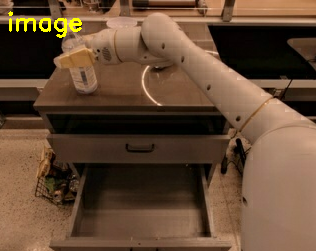
\includegraphics[width=\linewidth]{figures/sample_source_0000_bottle.png}
    \caption{Object blockage/reachability, source 0.}
  \end{subfigure}
  \hfill
  \begin{subfigure}[t]{0.48\linewidth}
    \centering
    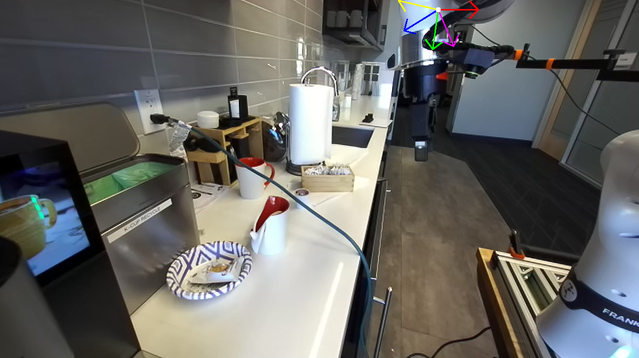
\includegraphics[width=\linewidth]{figures/sample_source_0368_directional_orientation.png}
    \caption{Directional orientation, source 368.}
  \end{subfigure}
  \vspace{3pt}

  \begin{subfigure}[t]{0.48\linewidth}
    \centering
    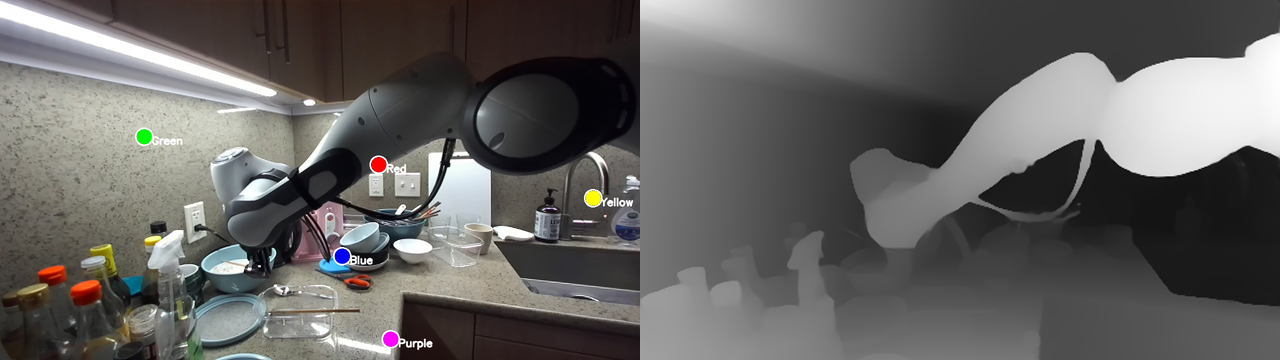
\includegraphics[width=\linewidth]{figures/sample_source_0407_depth_ordering.png}
    \caption{Depth/distance ordering, source 407.}
  \end{subfigure}
  \hfill
  \begin{subfigure}[t]{0.48\linewidth}
    \centering
    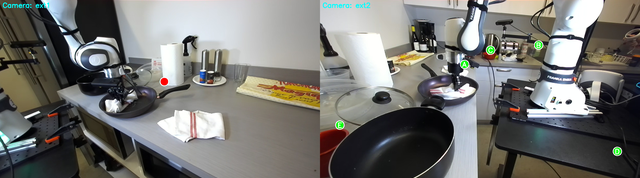
\includegraphics[width=\linewidth]{figures/sample_source_0408_cross_view.png}
    \caption{Cross-view correspondence, source 408.}
  \end{subfigure}
  \caption{Actual Robo2VLM examples used to ground the benchmark categories. The images show why aggregate VQA accuracy is insufficient: the benchmark mixes reachability judgments, end-effector directional orientation, depth ordering from overlaid points, and correspondence across camera views. The first panel also corresponds to the DeepSeek CoT failure in \cref{tab:evidence}, where the model treats the target bottle itself as an obstacle.}
  \label{fig:data-samples}
\end{figure*}

\textbf{Sanity probes.}
The scored runs are complemented by raw-generation probes over 20 spatial CoT examples per model. For each example, we ask the model to justify the correct answer on the original image, assess a deliberately wrong answer, assess the correct answer on a blank image, assess the correct answer on a shuffled mismatched image, and describe overlays without selecting an answer. A phrase-based heuristic labels each response as supporting, rejecting/insufficient, or unclear. These labels are for triage, not a substitute for manual grounding evaluation.

\textbf{Human performance evaluation.}
To complement the automated model evaluation, a human performance study was conducted on a subset of the benchmark. This analysis was motivated by the observation that the evaluated vision-language models exhibited only marginal performance differences across settings, prompting a closer inspection of the dataset itself. A manual review revealed that a subset of samples contains ambiguities, incomplete visual information, or inherently under-specified questions, which can make them challenging even for human annotators.

To quantify the impact of such issues, a random subset of 50 question–image pairs was selected from the curated dataset and presented to a group of human participants. The participants were asked to answer each question based solely on the provided image and task description, without access to external information or prior context.

\section{Implementation Provenance}
\label{sec:implementation}

\textbf{Implemented in this project.}
We implemented the Robo2VLM curation and post-processing pipeline, including the spatial/affordance/discarded taxonomy, deterministic subcategory rules, goal-state relabeling, and JSONL summaries. We also implemented the config-driven CLI around the evaluator, Slurm entrypoints, prompt-mode handling, option-letter extraction, subset loading by curated source index, RGB-depth image augmentation hooks, visual sanity controls, diagnostic prompt generation, and analysis summaries. The checked-in tests cover curation post-processing, config validation, and plotting/visualization utilities.

\textbf{External code and models.}
The underlying Robo2VLM dataset and original generation/fine-tuning code are external to our contribution and are used as the source benchmark~\cite{chen2025robo2vlm}. Inference uses vLLM and model-family prompt wrappers adapted from vLLM examples. The evaluated pretrained VLMs are external checkpoints, including Qwen2.5-VL~\cite{bai2025qwen25vl}, DeepSeek-VL2~\cite{wu2024deepseekvl2}, and poster-reported compact baselines. Optional RGB-depth images use an external monocular depth estimator. The curation labels were produced with an external hosted LLM API; our contribution is the taxonomy, prompting, validation, deterministic post-processing, and downstream evaluation logic.

\section{Experimental Setup}
\label{sec:setup}

The main raw-result matrix evaluates Qwen2.5-VL-3B-Instruct and DeepSeek-VL2-tiny on the spatial and affordance subsets, with zero-shot and CoT prompts. All audited runs use Robo2VLM-1 test images, RGB input, temperature 0.0, batch size 1, tensor parallel size 1, and 200 examples per subset. Zero-shot generations are capped at 128 tokens, while CoT runs allow longer responses. Additional poster-reported compact baselines are included in \cref{tab:poster}.

The evaluated tasks are five-way multiple choice, so uniform chance is 20\%. Response time is measured per generated answer. For prompt comparisons, we pair zero-shot and CoT results by question ID and count cases where zero-shot is correct but CoT is wrong, and vice versa.

\section{Results}
\label{sec:results}

\textbf{Qwen and DeepSeek evaluations}
\cref{tab:main-results} shows the main Qwen and DeepSeek matrix. Spatial reasoning is essentially unsolved in this setting: the best audited spatial result is 22.0\%, only two percentage points above five-way chance. Affordance results are stronger, but the subcategory analysis in \cref{tab:subcat} shows that this strength is mostly due to object blockage/reachability questions rather than stable grasp reasoning.

\begin{table}[htbp]
  \centering
  \resizebox{\columnwidth}{!}{%
  \begin{tabular}{@{}lcc@{}}
    \toprule
    \textbf{Model} & \textbf{Spatial ZS} & \textbf{Spatial CoT} \\
    \midrule
    Qwen2.5-VL-3B & \textbf{40/200, 20.0\%} (0.18s) & \textbf{39/200, 19.5\%} (4.90s) \\
    DeepSeek-VL2-tiny & \textbf{39/200, 19.5\%} (0.17s) & \textbf{44/200, 22.0\%} (0.74s) \\
    \midrule
    \midrule
    \textbf{Model} & \textbf{Affordance ZS} & \textbf{Affordance CoT} \\
    \midrule
    Qwen2.5-VL-3B & 131/200, 65.5\% (0.46s) & 128/200, 64.0\% (3.40s) \\
    DeepSeek-VL2-tiny & \textbf{144/200, 72.0\%} (0.14s) & \textbf{43/200, 21.5\%} (0.27s) \\
    \bottomrule
  \end{tabular}%
  }
  \caption{Main audited 200-example results. Cells report correct/total, accuracy, and average response time. Bold values mark the near-chance spatial results and the DeepSeek affordance zero-shot/CoT contrast.}
  \label{tab:main-results}
\end{table}

\textbf{Effect of Prompting Strategy: zero-shot vs. CoT.}
CoT changes behavior but does not reliably improve accuracy. For Qwen2.5-VL-3B, CoT slightly hurts both spatial and affordance performance: $-0.5$ percentage points on spatial and $-1.5$ on affordance. DeepSeek-VL2-tiny gains only $+2.5$ points on spatial, but collapses on affordance from 72.0\% zero-shot to 21.5\% CoT. In the paired DeepSeek affordance comparison, 114 examples are correct in zero-shot but wrong under CoT, while only 13 move from wrong to correct. This is the clearest evidence that reasoning traces can introduce systematic errors rather than merely exposing latent reasoning.

\begin{table}[htbp]
  \centering
  \resizebox{\columnwidth}{!}{%
  \begin{tabular}{@{}llccc@{}}
    \toprule
    \textbf{Model} & \textbf{Prompt} & \textbf{Directional orient.} & \textbf{Depth/order} & \textbf{Cross-view} \\
    \midrule
    Qwen2.5-VL-3B & ZS & \textbf{8/76, 10.5\%} & 24/91, 26.4\% & 8/33, 24.2\% \\
    Qwen2.5-VL-3B & CoT & 12/76, 15.8\% & 21/91, 23.1\% & 6/33, 18.2\% \\
    DeepSeek-VL2-tiny & ZS & 14/76, 18.4\% & 17/91, 18.7\% & 8/33, 24.2\% \\
    DeepSeek-VL2-tiny & CoT & 15/76, 19.7\% & 21/91, 23.1\% & 8/33, 24.2\% \\
    \midrule
    \midrule
    \textbf{Model} & \textbf{Prompt} & \textbf{Blockage/reach.} & \textbf{Grasp stability} & \\
    \midrule
    Qwen2.5-VL-3B & ZS & \textbf{105/132, 79.5\%} & 26/68, 38.2\% & \\
    Qwen2.5-VL-3B & CoT & \textbf{107/132, 81.1\%} & 21/68, 30.9\% & \\
    DeepSeek-VL2-tiny & ZS & \textbf{112/132, 84.8\%} & 32/68, 47.1\% & \\
    DeepSeek-VL2-tiny & CoT & \textbf{18/132, 13.6\%} & \textbf{25/68, 36.8\%} & \\
    \bottomrule
  \end{tabular}%
  }
  \caption{Subcategory breakdown for the audited 200-example spatial and affordance slices. Bold values mark the central findings: near-chance directional orientation, strong object blockage/reachability performance, and the DeepSeek CoT collapse on blockage/reachability.}
  \label{tab:subcat}
\end{table}

\begin{table}[t]
  \centering
  \small
  \setlength{\tabcolsep}{4pt}
  \begin{tabular}{@{}lcccc@{}}
    \toprule
    Model & Spatial ZS & Aff. ZS & Spatial CoT & Aff. CoT \\
    \midrule
    SmolVLM-2.2B & \textbf{20\%} & 23\% & 66\% & 47\% \\
    Phi-4-multimodal & \textbf{12\%} & 19\% & 40\% & 44\% \\
    \bottomrule
  \end{tabular}
  \caption{Additional compact-model results.}
  \label{tab:poster}
\end{table}

\textbf{Effect of Depth Information.}
Contrary to expectations, depth information did not show any improvement in model accuracy. Qwen2.5-VL-3B was benchmarked on a dataset of 2084 spatial reasoning examples, which were augmented by concatenating the depth image to the side of the original image. Evaluated with zero-shot prompting, accuracy actually decreased slightly to 18.3\% on RGB-depth images.

\textbf{Sanity probes results.}
\cref{tab:sanity} summarizes the raw image-understanding sanity probes. Both audited models reject blank images reliably, so the image channel is not entirely ignored. The more informative controls are wrong answers and shuffled images. Qwen supports a deliberately wrong answer in 16/20 cases and rejects only 3/20 shuffled-image controls. DeepSeek rejects all shuffled controls, but its correct-answer explanations are usually classified as unclear. These probes show why answer accuracy alone is not sufficient evidence for grounded robotics reasoning.

\begin{table*}[t]
  \centering
  \small
  \setlength{\tabcolsep}{4pt}
  \begin{tabular}{@{}lp{0.34\linewidth}p{0.23\linewidth}p{0.23\linewidth}@{}}
    \toprule
    Probe & Expected behavior & Qwen2.5-VL-3B & DeepSeek-VL2-tiny \\
    \midrule
    Correct answer & Support correct answer on original image & 12 supports, 8 unclear & \textbf{20 unclear} \\
    Wrong answer & Reject deliberately wrong answer & \textbf{16 supports}, 4 unclear & 3 rejects, 17 unclear \\
    Blank image & Reject image as insufficient & 20 rejects & 20 rejects \\
    Shuffled image & Reject mismatched image & \textbf{3 rejects}, 17 unclear & \textbf{20 rejects} \\
    Overlay description & Describe visual overlays without answering & 20 unclear & 20 unclear \\
    \bottomrule
  \end{tabular}
  \caption{Heuristic labels for 20 examples per probe type. Bold values mark behavior most relevant to the grounding claim: unclear correct-answer support, wrong-answer rationalization, and mismatched-image rejection or failure to reject.}
  \label{tab:sanity}
\end{table*}


\textbf{Human baseline.}
The resulting human performance provides an additional reference point for interpreting model results and for assessing benchmark validity. In particular, it helps determine whether incorrect model predictions stem from limitations in model reasoning or from ambiguities inherent in the benchmark itself. \cref{tab:human} indicates that VLMs outperform human participants in overall affordance understanding, with the most pronounced advantage observed in the grasp stability subcategory. In contrast, humans demonstrate stronger performance in spatial reasoning tasks. However, it is noteworthy that performance in the directional orientation subcategory remains close to chance level (five-way guessing), suggesting that both humans and models struggle with this aspect of spatial reasoning using the Robo2VLM dataset.

\begin{table*}[t]
  \centering
  \small
  \setlength{\tabcolsep}{4pt}
  \begin{tabular}{@{}lccc@{}}
    \toprule
    Spatial total & Directional orientation & Depth/distance ordering & Cross-view correspondence \\
    \midrule
    43.3\% & \textbf{26.9\%} & 52.5\% & 42.0\% \\
    \midrule
    Affordance total & Object blockage/reachability & Grasp stability & \\
    \midrule
    45.0\% & 63.3\% & \textbf{22.7\%} & \\
    \bottomrule
  \end{tabular}
  \caption{Human performance using a randomized 50 data-samples subset. Bold values mark the human categories closest to chance and therefore most indicative of benchmark difficulty or ambiguity.}
  \label{tab:human}
\end{table*}

\section{Discussion}
\label{sec:discussion}

\textbf{Aggregate benchmark scores can be misleading.}
The affordance subset appears substantially easier than spatial reasoning in the headline table, but \cref{tab:subcat} shows that this is not uniform affordance competence. Object blockage/reachability questions drive most of the score, while grasp stability remains below 50\% for every audited run. The bottle scene in \cref{fig:data-samples} illustrates the kind of visual judgment involved: the model must distinguish the target object, the robot arm, and possible obstructions rather than answer from the word ``obstacle'' alone. This matters for robotics because a robot that can answer obstacle questions from template cues may still fail to judge whether a grasp is physically stable.

\textbf{Spatial reasoning remains a critical weakness.}
The audited spatial results cluster around chance despite evaluating models with strong general visual-language capabilities~\cite{bai2025qwen25vl,wu2024deepseekvl2}. Directional orientation, depth/distance ordering, and cross-view correspondence questions all remain weak. The visual categories in \cref{fig:data-samples} show why these questions are nontrivial: colored overlays must be interpreted relative to camera geometry, robot pose, and multi-view alignment. The qualitative evidence in \cref{tab:evidence} shows one concrete failure mode: a CoT response infers camera distance from 2D point position, which is an unreliable shortcut for the tested views.

\textbf{CoT is an ablation, not a default improvement.}
CoT is often treated as a low-cost way to improve reasoning. Here, it is at best mixed. Qwen changes many individual decisions without improving aggregate accuracy. DeepSeek gains a small amount on spatial questions but fails dramatically on affordance CoT, especially object blockage/reachability. The first row of \cref{tab:evidence} shows the failure directly: in a bottle reachability question, zero-shot predicts the correct answer, while CoT treats the target bottle itself as an obstacle and changes to the wrong answer. This is not merely random noise; it matches the aggregate fall from 84.8\% to 13.6\% on object blockage/reachability.

\begin{table*}[t]
  \centering
  \small
  \setlength{\tabcolsep}{4pt}
  \begin{tabular}{@{}p{0.18\linewidth}p{0.30\linewidth}p{0.22\linewidth}p{0.22\linewidth}@{}}
    \toprule
    Claim tested & Example question & Observed outputs & Why it matters \\
    \midrule
    DeepSeek CoT can harm affordance reasoning &
    Is there any obstacle blocking the robot from reaching bottle? &
    Expected A. DeepSeek ZS: A, correct. DeepSeek CoT: D, wrong. CoT excerpt: ``presence of an object (bottle) ... may pose a challenge.'' &
    The reasoning trace confuses the target with an obstacle, explaining the object blockage/reachability collapse. \\
    \midrule
    CoT can use weak 2D shortcuts for depth &
    Which colored point is farthest from the camera? &
    Expected B. Qwen ZS: B, correct. Qwen CoT: D, wrong. CoT excerpt: ``distance ... inferred from their positions.'' &
    The explanation relies on image-plane position as a proxy for 3D distance. \\
    \midrule
    CoT can help individual cases without improving aggregate accuracy &
    Is there any obstacle blocking the robot from reaching chip bag? &
    Expected C. Qwen ZS: D, wrong. Qwen CoT: C, correct. CoT notes no obstacle between robot and chip bag. &
    This explains why per-example behavior changes substantially even when Qwen's aggregate CoT score decreases. \\
    \midrule
    Answer explanations can be ungrounded &
    Wrong-answer probe on a spatial question with correct answer A: Red but proposed answer B: Purple. &
    Qwen response: ``The proposed answer B: Purple is supported by the visible evidence.'' &
    The model can rationalize a deliberately wrong answer instead of rejecting it. \\
    \midrule
    Image mismatch detection differs by model &
    Shuffled-image probe with original correct answer A: Red. &
    Qwen: unclear description of the mismatched scene. DeepSeek: ``current image does not visibly support'' the answer. &
    The two models can have similar spatial accuracy while differing sharply in grounding diagnostics. \\
    \bottomrule
  \end{tabular}
  \caption{Representative evidence from the actual evaluation and sanity-probe artifacts. These examples are not additional metrics; they expose the failure mechanisms behind the aggregate findings.}
  \label{tab:evidence}
\end{table*}

\textbf{Grounded explanations need separate tests.}
The sanity probes reveal a distinction between answering and grounding. Qwen correctly rejects blank images, yet it also supports deliberately wrong answers and often fails to reject shuffled images. DeepSeek handles shuffled images better, but its explanations are often not phrased as explicit support for the known correct answer. The last two rows of \cref{tab:evidence} make this failure visible: the same evaluation setup can expose rationalization, mismatch sensitivity, and answer accuracy as separate properties. A benchmark that reports only multiple-choice accuracy would miss these behaviors.

\textbf{Limitations.}
The main raw-result matrix uses 200 examples per subset and file-order sampling. The sanity probe heuristic is coarse and should be followed by manual review before making fine-grained claims about explanation quality. The benchmark also inherits Robo2VLM's multiple-choice format, template distribution, and generated-answer assumptions. These limitations do not weaken the central diagnostic result: targeted slicing and controls expose failures that aggregate robotics VQA scores can hide.

The scope of the evaluation was constrained by available computational resources, limiting the study to relatively small VLMs. Since model scaling has been shown to improve performance across a range of reasoning tasks, it remains an open question whether larger models would exhibit stronger spatial and affordance reasoning abilities. Exploring this relationship constitutes an important avenue for future research.

\textbf{Flawed dataset.}
A key finding from the human evaluation is that performance is not consistently high even for human participants. Several samples were identified as overly ambiguous, under-specified, or otherwise too difficult to be reliably solved based on the provided image and question alone. This indicates that a non-negligible portion of the dataset does not constitute well-posed evaluation cases for spatial and affordance reasoning.

As a consequence, the benchmark in its current form cannot be directly used as-is for reliable model evaluation. Instead, it requires additional manual filtering and curation to isolate representative and well-defined task instances. Such handpicking of high-quality samples is necessary to ensure that the final benchmark accurately reflects the intended reasoning capabilities and provides a meaningful basis for comparing model performance.

\section{Conclusion}
\label{sec:conclusion}

This project adds a targeted diagnostic layer to Robo2VLM for evaluating spatial reasoning and affordance understanding in robotics VQA. The results show that current VLMs can appear competent on aggregate affordance questions while still failing grasp stability, depth/distance ordering, directional orientation, cross-view correspondence, and grounding checks. The report therefore supports a conservative recommendation: robotics VLM benchmarks should report ability-specific slices, prompt-mode ablations, concrete qualitative evidence, and image-grounding controls rather than relying on a single VQA accuracy number.

{
    \small
    \bibliographystyle{ieeenat_fullname}
    \bibliography{main}
}

\end{document}
